\chapter{تصنيف الحيوانات}\label{ch:g4:classifying-animals}

يحفظ متحف التاريخ الطبيعي ملايين \omterm{def:g1:animals-around-us:animal}{الحيوانات} --- أدراج خنافس، وقاعات
هياكل عظمية، وجرار أسماك. ومع ذلك يستطيع أمين المتحف أن يمشي إلى
أي واحد منها في دقائق. والسر ليس الذاكرة بل \emph{الترتيب}: فلكل
\omterm{def:g1:animals-around-us:animal}{حيوان} مكانه في نظام كبير من مجموعات داخل مجموعات، مبني على قواعد
الفرز في \cref{ch:g3:sorting-living-things} --- وهذه السنة نتعلم
كيف يعمل ذلك النظام.

\section{مجموعات داخل مجموعات}

\begin{definition}[التصنيف]\label{def:g4:classifying-animals:classification}
أن \emph{تصنّف}\index{تصنيف} الكائنات الحية هو أن تفرزها بصفات
الجسم المشتركة في مجموعات، وأن تفرز تلك المجموعات في مجموعات أكبر
--- أي \emph{مجموعات متداخلة}\index{مجموعات متداخلة}، كالصناديق في
الصناديق. والترتيب كله \emph{نظام تصنيف}\index{نظام تصنيف}.
\end{definition}

\begin{example}[عناوين القطة]\label{ex:g4:classifying-animals:cat}
قطة واحدة، وعناوين متداخلة عدة: فالقطة \emph{ثديي} (\omterm{def:g1:animals-around-us:covering}{فرو}، \omterm{def:g2:animals-grow-up:born}{وحليب}
للصغار)؛ وكل ثديي \emph{\omterm{def:g4:classifying-animals:vertebrate}{فقاري}} (هيكل داخلي فيه \omterm{def:g4:classifying-animals:vertebrate}{عمود فقري})؛ وكل
\omterm{def:g4:classifying-animals:vertebrate}{فقاري} \emph{\omterm{def:g1:animals-around-us:animal}{حيوان}}. القطة داخل \omterm{prop:g3:sorting-living-things:groups}{الثدييات}، \omterm{prop:g3:sorting-living-things:groups}{والثدييات} داخل
\omterm{def:g4:classifying-animals:vertebrate}{الفقاريات}، \omterm{def:g4:classifying-animals:vertebrate}{والفقاريات} داخل \omterm{def:g1:animals-around-us:animal}{الحيوانات}: كل صندوق يقع داخل صندوق
أكبر منه.
\end{example}

\begin{definition}[الفقاريات واللافقاريات]\label{def:g4:classifying-animals:vertebrate}
\emph{الفقاري}\index{فقاري} \omterm{def:g1:animals-around-us:animal}{حيوان} له هيكل داخلي مبني حول
\emph{عمود فقري}\index{عمود فقري} --- كالعمود الذي تحسّسته في
\cref{ex:g3:bones-and-muscles:feel}. \omterm{def:g1:animals-around-us:animal}{والحيوان} الذي لا عمود فقري
له \emph{لافقاري}\index{لافقاري}: \omterm{prop:g3:sorting-living-things:groups}{كالحشرات}، والعناكب، والحلزونات،
والديدان، وقناديل البحر --- وهي السواد الأعظم من \omterm{def:g1:animals-around-us:animal}{الحيوانات} كلها.
\end{definition}

\begin{omfigure}
\begin{tikzpicture}[scale=0.86]
  % outer box: animals
  \draw[thick, omExo] (-0.3,-0.5) rectangle (12.1,4.4);
  \node[font=\small\bfseries, omExo] at (0.9,4.1) {حيوانات};
  % vertebrates box
  \draw[thick, omDef, fill=omDef!4] (0.0,-0.2) rectangle (7.4,3.6);
  \node[font=\small\bfseries, omDef] at (1.35,3.3) {فقاريات};
  \node[font=\footnotesize, omDef] at (2.6,2.85) {(عمود فقري في الداخل)};
  % five classes
  \foreach \x/\name in {0.25/أسماك, 1.65/برمائيات, 3.05/زواحف,
      4.45/طيور, 5.85/ثدييات} {
    \draw[thick, omMeth, fill=omMeth!7] (\x,0.1) rectangle ({\x+1.3},2.4);
    \node[font=\footnotesize, rotate=90] at ({\x+0.65},1.25) {\name};
  }
  % invertebrates box
  \draw[thick, omProp, fill=omProp!5] (7.8,-0.2) rectangle (11.9,3.6);
  \node[font=\small\bfseries, omProp] at (9.2,3.3) {لافقاريات};
  \node[font=\footnotesize, align=center] at (9.85,1.4)
    {حشرات، وعناكب،\\ وحلزونات، وديدان،\\ وقناديل بحر، \dots\\[3pt]
     (أكثر الحيوانات!)};
\end{tikzpicture}

{\small صناديق في صناديق: \omterm{prop:g4:classifying-animals:classes}{طوائف} \omterm{def:g4:classifying-animals:vertebrate}{الفقاريات} الخمس تكوّن معًا صندوقًا
واحدًا، يقع بجانب صندوق \omterm{def:g4:classifying-animals:vertebrate}{اللافقاريات} الأشد ازدحامًا بكثير، داخل
صندوق \omterm{def:g1:animals-around-us:animal}{الحيوانات} كلها.}
\end{omfigure}

\section{طوائف الفقاريات الخمس}

\begin{proposition}[طوائف الفقاريات الخمس]\label{prop:g4:classifying-animals:classes}
تُصنَّف \omterm{def:g4:classifying-animals:vertebrate}{الفقاريات} في خمس مجموعات كبرى تسمى
\emph{طوائف}\index{طائفة}:
\begin{enumerate}
  \item \emph{\omterm{prop:g3:sorting-living-things:groups}{الأسماك}}: حراشف، وزعانف، وتنفس في الماء --- كالسلمون
        المرقط والقرش والسردين؛
  \item و\emph{البرمائيات}\index{برمائي}: \omterm{def:g1:the-five-senses:sense}{جلد} عارٍ رطب، \omterm{def:g2:animals-grow-up:born}{وبيض} في
        الماء، وطفولة شرغوفية --- كالضفدع والعلجوم والسمندل؛
  \item و\emph{الزواحف}\index{زاحف}: \omterm{def:g1:the-five-senses:sense}{جلد} جاف حرشفي، وأكثرها يضع
        بيضًا مقشورًا على اليابسة --- كالسحلية والأفعى والسلحفاة
        والتمساح؛
  \item و\emph{\omterm{prop:g3:sorting-living-things:groups}{الطيور}}: \omterm{def:g1:animals-around-us:covering}{ريش}، ومنقار، \omterm{def:g2:animals-grow-up:born}{وبيض} مقشور --- كالشحرور
        والنعامة والبطريق؛
  \item و\emph{\omterm{prop:g3:sorting-living-things:groups}{الثدييات}}: \omterm{def:g1:animals-around-us:covering}{فرو} أو شعر، وصغار تُرضع \omterm{def:g2:animals-grow-up:born}{الحليب} ---
        كالقطة والحوت والخفاش والإنسان.
\end{enumerate}
\end{proposition}
\admitted

\begin{example}[فرز شحنة حديقة حيوان]\label{ex:g4:classifying-animals:zoo}
تصل ست صناديق: ثعبان أصلة (\omterm{def:g1:the-five-senses:sense}{جلد} جاف حرشفي، \omterm{def:g2:animals-grow-up:born}{وبيض} مقشور --- زاحف)،
وعلجوم (\omterm{def:g1:the-five-senses:sense}{جلد} عارٍ رطب --- برمائي)، وبطريق (\omterm{def:g1:animals-around-us:covering}{ريش} --- طائر)، وقرش
(زعانف وغلاصم --- سمكة)، ودلفين (\omterm{def:g2:animals-grow-up:born}{حليب} لعجله --- ثديي)، وصندوق
حلزونات عملاقة (لا \omterm{def:g4:classifying-animals:vertebrate}{عمود فقري} لها البتة --- \omterm{def:g4:classifying-animals:vertebrate}{لافقاريات}، ليست في أي
طائفة من \omterm{def:g4:classifying-animals:vertebrate}{الفقاريات}).
\end{example}

\begin{remark}[زاحف أم برمائي؟]\label{rem:g4:classifying-animals:confusion}
السحالي والسمادل تتشابه لأول وهلة --- أربع \omterm{def:g1:my-body:parts}{أرجل} وذنب طويل. \omterm{def:g1:the-five-senses:sense}{والجلد}
هو الذي يقرر: \omterm{def:g1:the-five-senses:sense}{فجلد} السحلية جاف حرشفي، \omterm{def:g1:the-five-senses:sense}{وجلد} السمندل رطب عارٍ؛ \omterm{def:g2:animals-grow-up:born}{وبيض}
السحلية مقشور يوضع على اليابسة، \omterm{def:g2:animals-grow-up:born}{وبيض} السمندل عارٍ يوضع في الماء.
الظل نفسه، وطائفتان مختلفتان.
\end{remark}

\section{استعمال نظام التصنيف}

\begin{method}[وضع فقاري في طائفته]\label{met:g4:classifying-animals:place}
اسأل الأسئلة بالترتيب، وقف عند أول نعم:
\begin{enumerate}
  \item أله \omterm{def:g1:animals-around-us:covering}{ريش}؟ --- إذن طائر.
  \item أله \omterm{def:g1:animals-around-us:covering}{فرو} أو شعر (أو \omterm{def:g2:animals-grow-up:born}{حليب} للصغار)؟ --- إذن ثديي.
  \item أجلده جاف حرشفي؟ --- إذن زاحف.
  \item أجلده رطب عارٍ وطفولته شرغوفية؟ --- إذن برمائي.
  \item أله زعانف وغلاصم وحياة في الماء؟ --- إذن سمكة.
\end{enumerate}
فإن لم يكن له \omterm{def:g4:classifying-animals:vertebrate}{عمود فقري} البتة، فهو \omterm{def:g4:classifying-animals:vertebrate}{لافقاري}، ولا تنطبق عليه هذه
الأسئلة.
\end{method}

\begin{proposition}[ما تعطيه الطائفة مجانًا]\label{prop:g4:classifying-animals:free}
معرفة طائفة \omterm{def:g1:animals-around-us:animal}{الحيوان} معرفة لحزمة من الحقائق قبل النظر: فإذا قيل لك
``إنه ثديي'' فحسب، توقّعت منذ الآن فروًا، وحليبًا للصغار، وصغارًا
تولد حية --- كما هي حال \omterm{prop:g3:sorting-living-things:groups}{الثدييات} كلها تقريبًا. وذلك التوفير هو
مقصود \omterm{def:g4:classifying-animals:classification}{التصنيف} كله: تعلَّم المجموعة مرة، فيصلك كل فرد منها معروفًا
نصف المعرفة.
\end{proposition}
\admitted

\begin{example}[وصول نوع جديد]\label{ex:g4:classifying-animals:new}
ما زال علماء الطبيعة يكتشفون \omterm{def:g1:animals-around-us:animal}{حيوانات} لم تُرَ من قبل. فحين يُعثر
على \omterm{def:g1:animals-around-us:animal}{حيوان} جديد شبيه بالخفاش له \omterm{def:g1:animals-around-us:covering}{فرو} \omterm{def:g2:animals-grow-up:born}{وحليب}، يُوضع في \omterm{prop:g3:sorting-living-things:groups}{الثدييات}
مباشرة --- ويتوقع علماء الأحياء في الحال عمودًا فقريًّا، وقلبًا ذا
أربع حجرات، ودمًا حارًّا، قبل أن يُتحقق من شيء من ذلك. \omterm{def:g4:classifying-animals:classification}{فنظام
التصنيف} يعطي تنبؤات.
\end{example}

\begin{remark}[نحو شجرة النسب]\label{rem:g4:classifying-animals:tree}
لماذا يسافر \omterm{def:g1:animals-around-us:covering}{الفرو} \omterm{def:g2:animals-grow-up:born}{والحليب} \omterm{def:g3:bones-and-muscles:skeleton}{والعمود الفقري} معًا بهذا الوفاء؟ الجواب
الكامل --- وهو أن أفراد المجموعة يرثون صفاتهم المشتركة من أسلاف
مشتركين --- ينتمي إلى حكاية القرابة والتطور، وستُتناول في سنوات
لاحقة. أما الآن فالصناديق المتداخلة تعمل ببساطة، وتعمل عملًا رائعًا.
\end{remark}

\begin{omfigure}
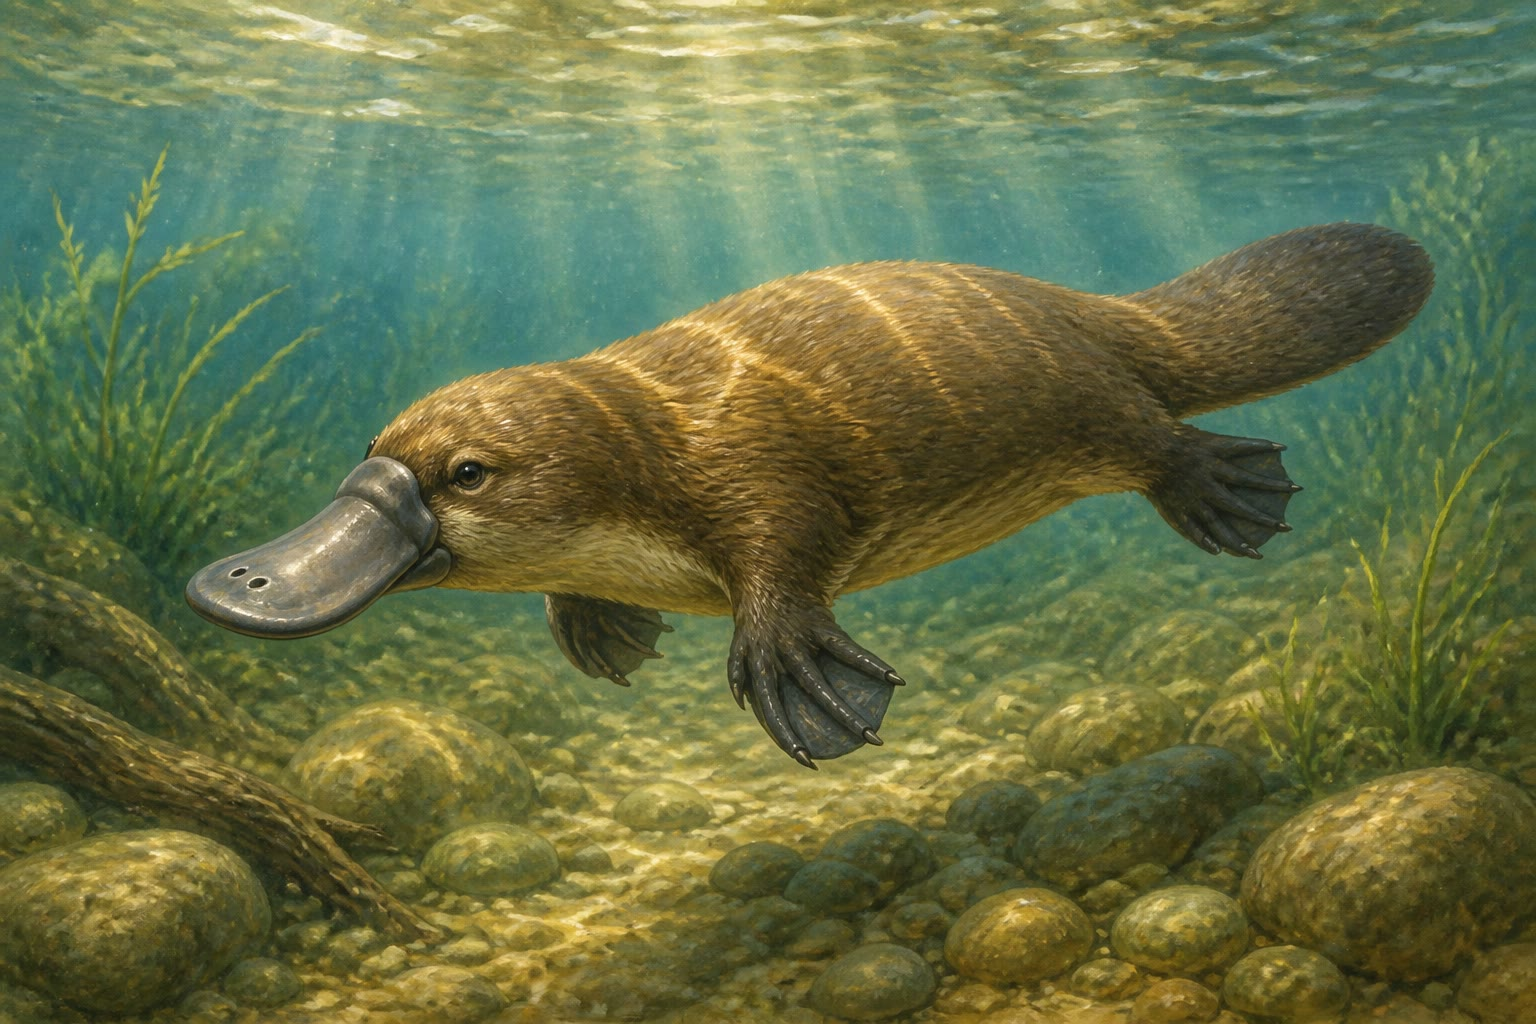
\includegraphics[width=0.6\linewidth]{images/book1/ai/g4-classify-platypus.jpg}

{\small صداع المصنِّف المفضل: \omterm{def:g1:animals-around-us:covering}{فرو} \omterm{def:g2:animals-grow-up:born}{وحليب}، لكن منقارًا وقدمين
مكفوفتين --- وبيضًا. منقار البط (انظر التمرين الأخير) يختبر
الطريقة كلها.}
\end{omfigure}

\section{تمارين}

\begin{exercise}[$\star$]\label{exo:g4:classifying-animals:1}
ما \omterm{def:g4:classifying-animals:vertebrate}{الفقاري}؟ وما \omterm{def:g4:classifying-animals:vertebrate}{اللافقاري}؟ أعطِ مثالين على كل واحد.
\end{exercise}

\begin{exercise}[$\star$]\label{exo:g4:classifying-animals:2}
سمِّ \omterm{prop:g4:classifying-animals:classes}{طوائف} \omterm{def:g4:classifying-animals:vertebrate}{الفقاريات} الخمس بصفاتها المميزة.
\end{exercise}

\begin{exercise}[$\star$]\label{exo:g4:classifying-animals:3}
ضع كل \omterm{def:g1:animals-around-us:animal}{حيوان} في مكانه: السردين، والتمساح، والسمندل، والنعامة،
والحوت، ودودة الأرض.
\end{exercise}

\begin{exercise}[$\star$]\label{exo:g4:classifying-animals:4}
اكتب عناوين القطة المتداخلة، من أصغر صندوق إلى أكبره، كما في
\cref{ex:g4:classifying-animals:cat}.
\end{exercise}

\begin{exercise}[$\star$]\label{exo:g4:classifying-animals:5}
السحلية والسمندل يتشابهان. فأي صفتين تفصلان بين طائفتيهما؟
\end{exercise}

\begin{exercise}[$\star$]\label{exo:g4:classifying-animals:6}
أي مجموعة تضم السواد الأعظم من \omterm{def:g1:animals-around-us:animal}{الحيوانات} كلها؟ سمِّ أربعة من
أفرادها.
\end{exercise}

\begin{exercise}[$\star$]\label{exo:g4:classifying-animals:7}
طبّق \cref{met:g4:classifying-animals:place} بصوت عالٍ على
البطريق وعلى الدلفين، سؤالًا سؤالًا.
\end{exercise}

\begin{exercise}[$\star$]\label{exo:g4:classifying-animals:8}
قيل لك فحسب: ``هذا \omterm{def:g1:animals-around-us:animal}{الحيوان} طائر.'' عدّد ثلاثة أشياء تتوقعها الآن
من غير أن تنظر، وفق \cref{prop:g4:classifying-animals:free}.
\end{exercise}

\begin{exercise}[$\star\star$]\label{exo:g4:classifying-animals:9}
الحوت لا شعر له تقريبًا وهو يعيش عيش السمك. استعمل
\cref{met:g4:classifying-animals:place}
و\cref{ex:g3:sorting-living-things:surprises} لتشرح لماذا هو ثديي
مع ذلك --- ولماذا لم تكن ``يعيش في البحر'' صفة \omterm{def:g4:classifying-animals:classification}{تصنيف} قط.
\end{exercise}

\begin{exercise}[$\star\star$]\label{exo:g4:classifying-animals:10}
الأفعى لا \omterm{def:g1:my-body:parts}{أرجل} لها، ولا \omterm{def:g1:my-body:parts}{أرجل} لدودة الأرض كذلك. فلماذا كانت إحداهما
زاحفًا فقاريًّا والأخرى لافقاريًّا؟ وأي صفة واحدة تعلو على غياب
\omterm{def:g1:my-body:parts}{الأرجل}؟
\end{exercise}

\begin{exercise}[$\star\star\star$]\label{exo:g4:classifying-animals:11}
حيّر منقار البط علماء الطبيعة: \omterm{def:g1:animals-around-us:covering}{فرو} \omterm{def:g2:animals-grow-up:born}{وحليب}، ومع ذلك يضع بيضًا
مقشورًا. فأي طائفة انتصرت، ولماذا؟ وعلام يدل هذا اللغز في شأن
\omterm{def:g4:classifying-animals:classification}{التصنيف} \emph{بحزم} من الصفات لا بصفة واحدة؟
\end{exercise}
